\begin{frame}
    \frametitle{Energy for the future}
        \begin{columns}
            \column[t]{5cm}

            \begin{quote}
                    Cheap and abundant nuclear energy is no longer a luxury; it will eventually be a necessity for the maintenance of the human condition. -- Alvin Weinberg
            \end{quote}

            %From \textit{The Age of Substitutability} by Goeller and Weinberg: energy is the ultimate limiting resource of future society.

            \begin{center}
                    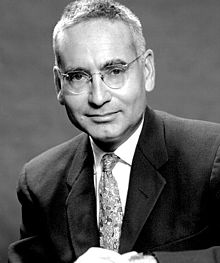
\includegraphics[height=0.3\textheight]{weinberg}
            \end{center}
            \column[t]{5cm}

            Molten salt reactors offer a convincing solution to the problem of fossil fuels.

            \begin{itemize}
                \item{Potentially much cheaper than normal nuclear}
                \item{Make meltdowns impossible}
                \item{Better natural resource utilization}
            \end{itemize}

        \end{columns}
\end{frame}

\begin{frame}
  \frametitle{MSR Comparison}
  
  \begin{columns}
      \column[t]{5cm}
      \textbf{Topaz Solar Farm}

      \begin{itemize}
          \item{9.5 sq. mi of California desert}

          \item{Max output of 550 MW(e), on average makes 132 MW(e)}

          \item{\$2.5B construction}
      \end{itemize}

      \begin{figure}[h]
          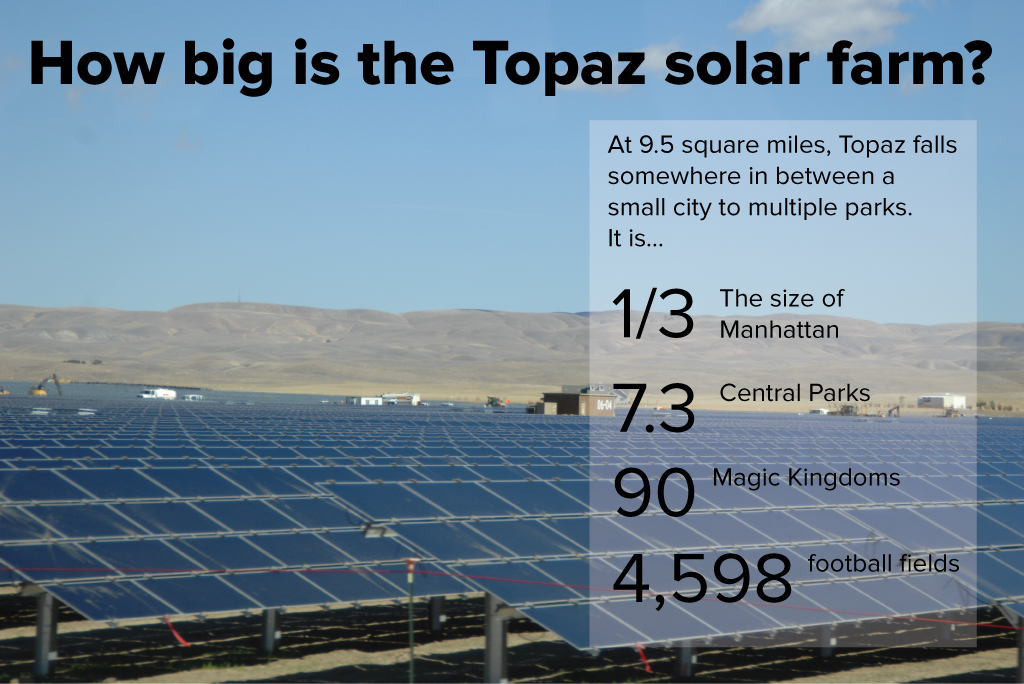
\includegraphics[width=\textwidth]{topaz}
          \caption{Topaz solar farm in California, credit GigaOM media}
      \end{figure}

      \column[t]{5cm}
      \textbf{Terrestrial Energy IMSR concept}

      \begin{itemize}
          \item{About 300 MW(e) output, more than double Topaz farm}

          \item{Initial cost estimates rank IMSR cheaper than coal}
      \end{itemize}
      \begin{figure}[h]
          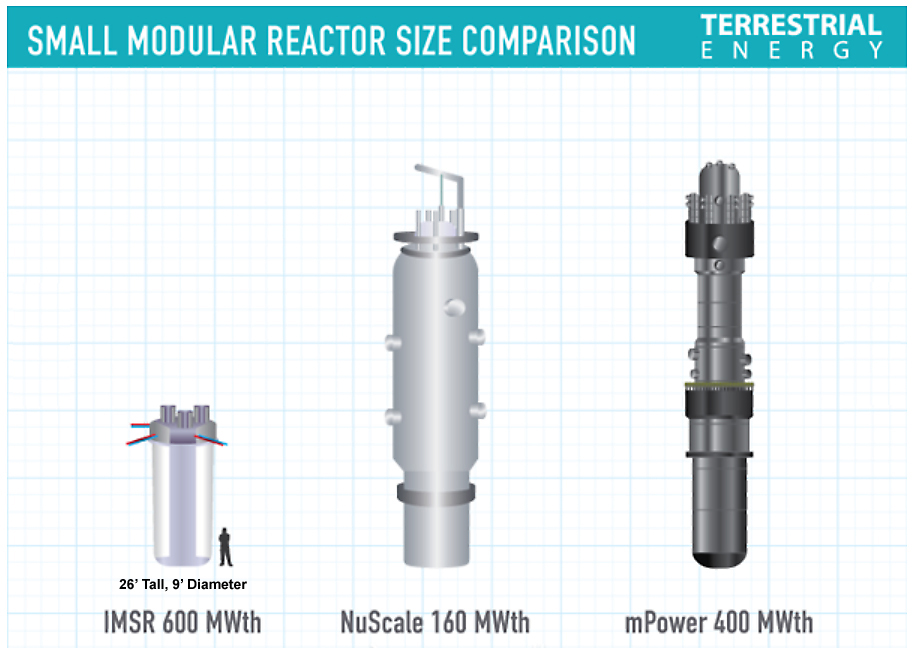
\includegraphics[width=\textwidth]{IMSR}
          \caption{IMSR and some other small nuclear designs, credit Terrestrial Energy}
      \end{figure}
  \end{columns}

\end{frame}
